\documentclass[border=6pt]{standalone}
\usepackage{tikz}
\usepackage[edges]{forest}
\usetikzlibrary{arrows.meta,positioning,calc,decorations.pathreplacing,shapes.geometric}
\begin{document}
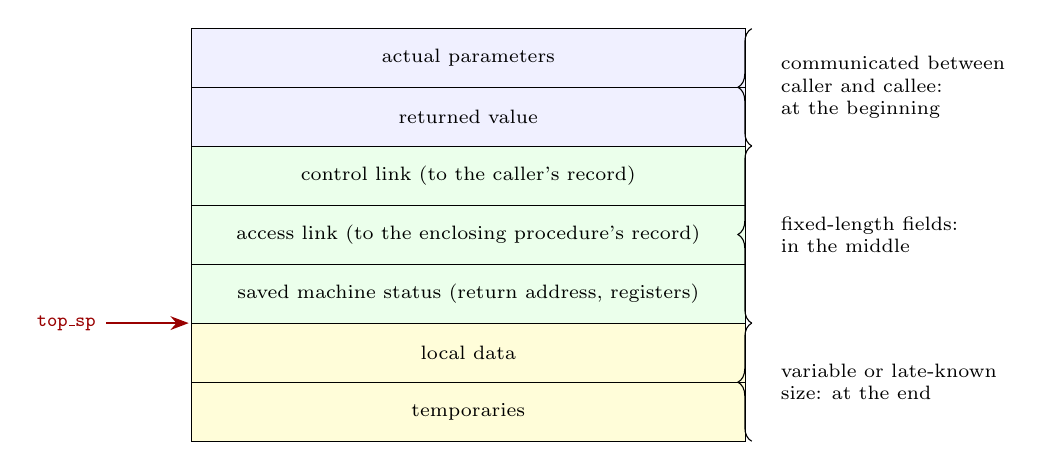
\begin{tikzpicture}[>=Stealth,font=\small,
  cell/.style={draw,minimum width=7.0cm,text width=6.8cm,minimum height=0.75cm,align=center,font=\scriptsize}]
\node[cell,fill=blue!6]  (c1) at (0,0) {actual parameters};
\node[cell,fill=blue!6]  (c2) at (0,-0.75) {returned value};
\node[cell,fill=green!8] (c3) at (0,-1.5) {control link (to the caller's record)};
\node[cell,fill=green!8] (c4) at (0,-2.25) {access link (to the enclosing procedure's record)};
\node[cell,fill=green!8] (c5) at (0,-3.0) {saved machine status (return address, registers)};
\node[cell,fill=yellow!15] (c6) at (0,-3.75) {local data};
\node[cell,fill=yellow!15] (c7) at (0,-4.5) {temporaries};
\draw[decorate,decoration={brace,amplitude=5pt,mirror}] (3.6,0.37) -- node[right=7pt,font=\scriptsize,align=left]{communicated between\\caller and callee:\\at the beginning} (3.6,-1.12);
\draw[decorate,decoration={brace,amplitude=5pt,mirror}] (3.6,-1.12) -- node[right=7pt,font=\scriptsize,align=left]{fixed-length fields:\\in the middle} (3.6,-3.37);
\draw[decorate,decoration={brace,amplitude=5pt,mirror}] (3.6,-3.37) -- node[right=7pt,font=\scriptsize,align=left]{variable or late-known\\size: at the end} (3.6,-4.87);
\draw[->,thick,red!60!black] (-4.6,-3.37) node[left,font=\scriptsize]{\texttt{top\_sp}} -- (-3.55,-3.37);
\end{tikzpicture}
\end{document}
